\documentclass[12pt,oneside,letterpaper]{article}

% graphicx package, useful for including eps and pdf graphics
\usepackage{graphicx}
\DeclareGraphicsExtensions{.pdf,.png,.jpg}

% basic packages
\usepackage{color}
\usepackage{parskip}
\usepackage{float}

% hyperref
\usepackage{hyperref}

% text layout
\usepackage{geometry}
\geometry{textwidth=15cm} % 15.25cm for single-space, 16.25cm for double-space
\geometry{textheight=22cm} % 22cm for single-space, 22.5cm for double-space

% helps to keep figures from being orphaned on a page by themselves
\renewcommand{\topfraction}{0.85}
\renewcommand{\textfraction}{0.1}

% bold the 'Figure #' in the caption and separate it with a period
% Captions will be left justified
\usepackage[labelfont=bf,labelsep=period,font=small]{caption}

% review layout with double-spacing
%\usepackage{setspace}
%\doublespacing
%\captionsetup{labelfont=bf,labelsep=period,font=doublespacing}

% cite package, to clean up citations in the main text. Do not remove.
\usepackage{cite}
%\renewcommand\citeleft{(}
%\renewcommand\citeright{)}
%\renewcommand\citeform[1]{\textsl{#1}}

% Remove brackets from numbering in list of References
\renewcommand\refname{\large References}
\makeatletter
\renewcommand{\@biblabel}[1]{\quad#1.}
\makeatother

\usepackage{authblk}
\renewcommand\Authands{ \& }
\renewcommand\Authfont{\normalsize \bf}
\renewcommand\Affilfont{\small \normalfont}
\makeatletter
\renewcommand\AB@affilsepx{, \protect\Affilfont}
\makeatother

% notation
\usepackage{amsmath}
\usepackage{amssymb}

%%% TITLE %%%
\title{\vspace{1.0cm} \Large \bf
    Forecasting SARS-CoV-2 clade success from deep mutational scanning
}

\author[1,2,$\dagger$, *]{Marlin D.\ Figgins}
\author[3,4, $\dagger$]{Cornelius Roemer}
\author[5, 6]{Jesse D. Bloom}
\author[1,5]{Trevor Bedford}

\affil[1]{Vaccine and Infectious Disease Division, Fred Hutchinson Cancer Research Center, Seattle, WA, USA}

\affil[2]{Department of Applied Mathematics, University of Washington, Seattle, WA, USA}

\affil[3]{Swiss Institute of Bioinformatics, Basel, Switzerland}

\affil[4]{Biozentrum, University of Basel, Basel, Switzerland}

\affil[5]{Basic Sciences Division and Computational Biology Program, Fred Hutchinson Cancer Center, Seattle, Washington, USA}

\affil[6]{Howard Hughes Medical Institute, Seattle, WA, USA}

\affil[$\dagger$]{These authors contributed equally to this work.}

\affil[*]{Corresponding author: mfiggins@uw.edu}

\date{\today}

\begin{document}

\maketitle

%%% ABSTRACT %%%
\begin{abstract}
Todo
\end{abstract}

%%% INTRODUCTION %%%
\section*{Introduction}

Over the course of the COVID-19 pandemic, genetic variants have emerged leading to large waves of infection (Omicron, XBB .etc) and significant turnover in the SARS-CoV-2 viral population.
Successful emerging variants are thought to succeed by escaping prior infection and vaccine-derived immunity though the accumulation of immune escaping mutations.

Various methods have been developed to access the escape potential of variant viruses such as titer models and deep mutational scanning.
However, these estimates of immune escape are typically derived in the lab and describe immunity escape of a viral variant against a particular immune background.

Though there is some work demonstrating that molecular estimates of immune escape correlate with population-level success, it is unclear how these escape scores factor into and predict larger success of genetic variants at the level of population frequency and variant turnover.
Theory predicts that population-level relative fitnesses should be a function of both these escape scores against particular immune backgrounds and the distribution of these backgrounds in the population.

On the side of population frequency predictions, fitness models have a found a use for short-term forecasts.
The simplest form of these models rely solely on sequence count or frequency data to make estimate relative fitness for variants.
However, these models appear to have trouble in forecasting in the medium and long-term due to a short effective forecast horizon, perhaps caused by variant emergence or time-dependence in relative fitness. 
Many purely statistical approaches have been developed to improve the ability to forecast and fit variant frequency data. 
One such example is hierarchical modeling or partial pooling of variant relative fitness which has been shown [Rockfeller].

However, modeling the relationship between molecular estimates of fitness and  population data is also a viable way forward and may be useful for explaining population level dynamics for SARS-CoV-2 variants.

Similar approaches of using molecular and phylogeny-based features for longer-term frequency forecast have been used in influenza to varying success.

Additionally, incorporation of external data for validation of estimated growth advantage has occurred.

Despite the existence of molecular estimates of immune escape exist, there’s little work combining these for forecasting of variant success in the future.

First, we show that escape scores and RBD ACE-2 binding computed from DMS are associated with higher growth advantages in emerging Pango lineages.
We then combine existing data into a new model to jointly estimate variant growth advantages accounting for evolutionary relationships between viruses and enable prediction of new variants based on this phylogenetic structure.
We also introduce a fully Bayesian model of variant growth advantages which incorporates both phylogenetic structure in its estimate to provide informed priors of a variant's relative fitness using molecular estimates of immune escape and its phylogenetic placement.
We then apply this work to identify likely escape candidates from BA.2 derived immunity and repeat this analysis for XBB.1.5.

%%% RESULTS %%%
\section*{Results}

\paragraph{Introduction to deep mutational scanning and frequency models}%

\paragraph{Molecular estimates explain relative fitness changes}%
(Figure~\ref{binding-escape-score-growth-advantage-innovations}).

\begin{figure}[h]
	\centering
	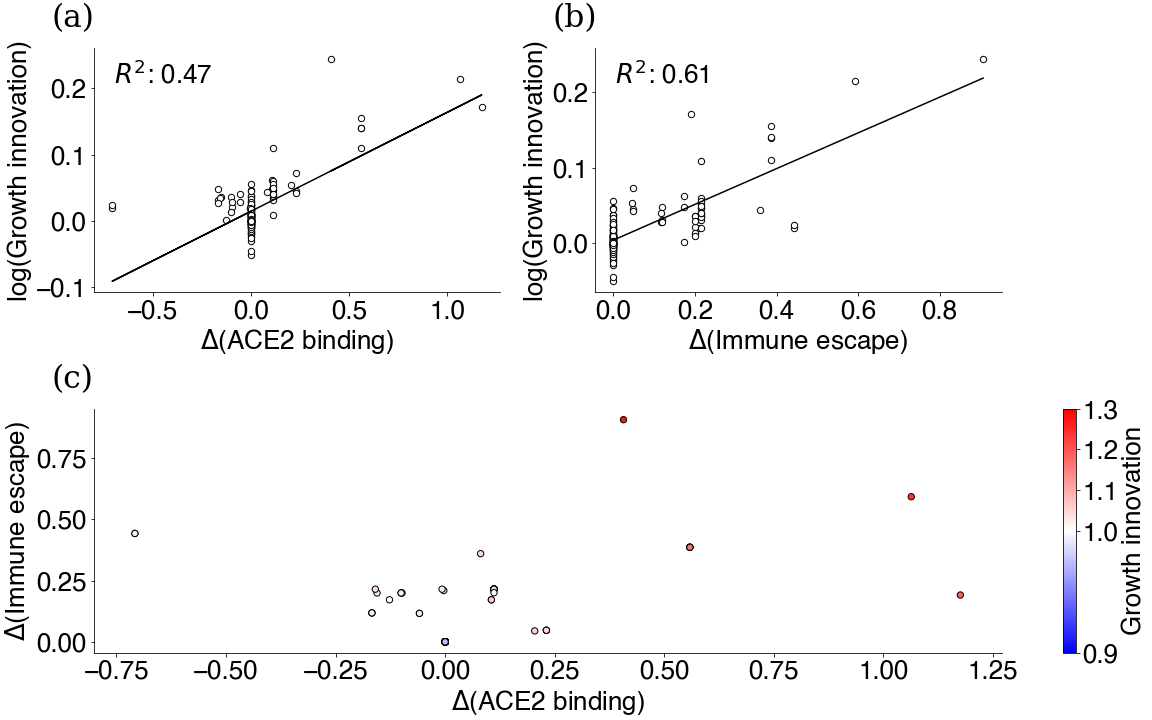
\includegraphics[width=1.0\textwidth]{figures/binding-escape-score-growth-advantage-innovations}
	\caption{\textbf{Correlation between changes in ACE-2 binding, immune escape and MLR growth advantage.}
        (a) Correlating log(growth advantage innovation) and change in ACE-2 binding. 
        (b) Correlating ... and change in immune escape.
        (c) Comparing predicted growth advantage from multiple regression to estimated growth advantage from innovation MLR model.
	}
	\label{binding-escape-score-growth-advantage-innovations}
\end{figure}

\begin{figure}[h]
	\centering
	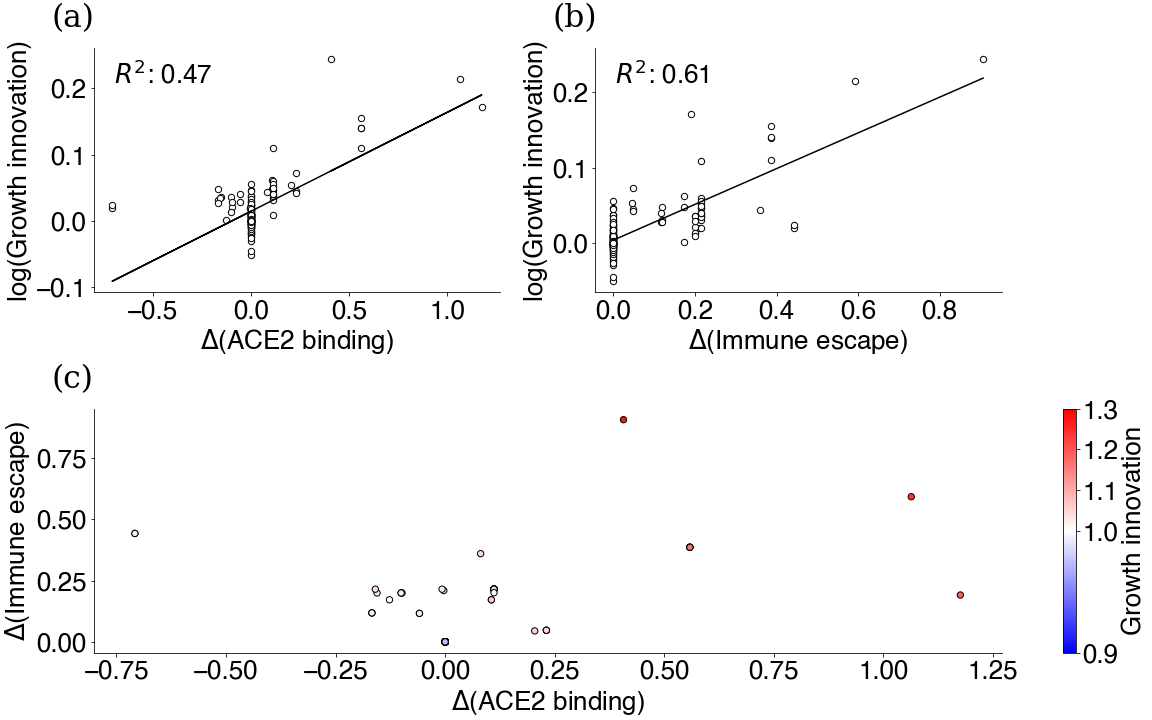
\includegraphics[width=1.0\textwidth]{figures/binding-escape-score-growth-advantage-innovations}
	\caption{\textbf{Correlation between changes in ACE-2 binding, immune escape and MLR growth advantage.}
        (a) Correlating log(growth advantage innovation) and change in ACE-2 binding. 
        (b) Correlating ... and change in immune escape.
        (c) Comparing predicted growth advantage from multiple regression to estimated growth advantage from innovation MLR model.
	}
	\label{binding-escape-score-growth-advantage-innovations-2}
\end{figure}

\begin{figure}[h]
	\centering
	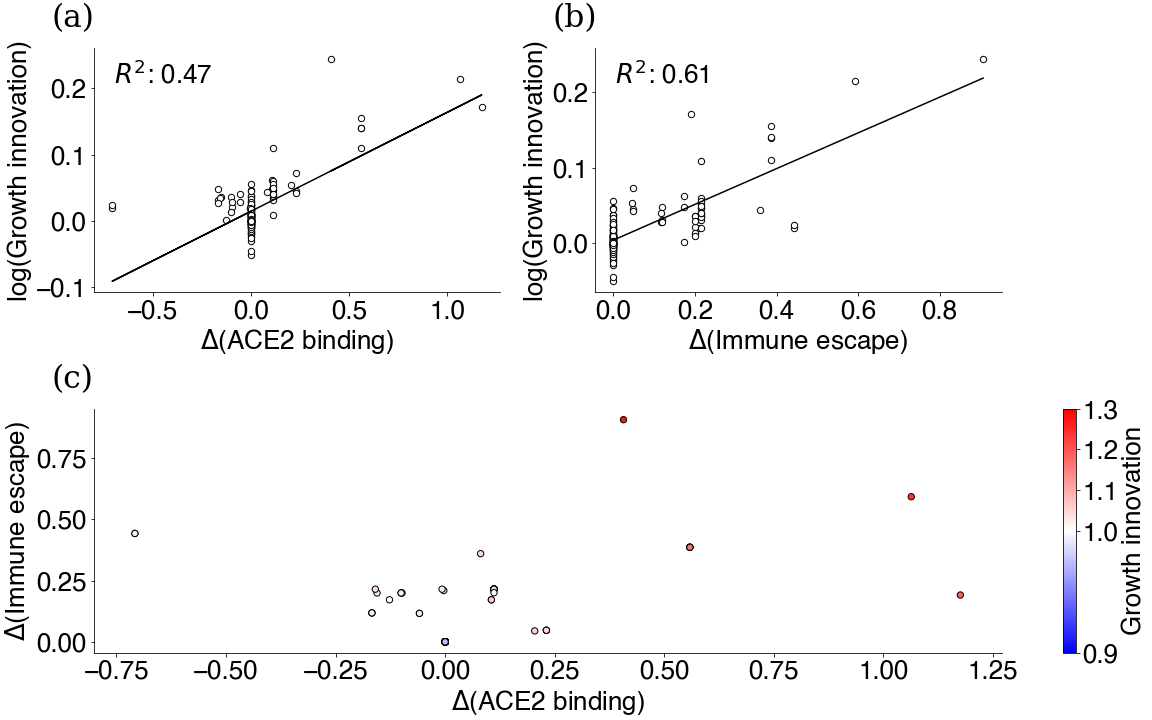
\includegraphics[width=1.0\textwidth]{figures/binding-escape-score-growth-advantage-innovations}
	\caption{\textbf{Correlation between changes in ACE-2 binding, immune escape and MLR growth advantage.}
        (a) Correlating log(growth advantage innovation) and change in ACE-2 binding. 
        (b) Correlating ... and change in immune escape.
        (c) Comparing predicted growth advantage from multiple regression to estimated growth advantage from innovation MLR model.
	}
	\label{binding-escape-score-growth-advantage-innovations-3}
\end{figure}


%%% DISCUSSION %%%
\section*{Discussion}

Need to update calculator and data set

Limitations in calculator itself

Generating of immune subgroups from calculator

Limits in calculator computation


%%% METHODS %%%
\section*{Methods}

\paragraph{Generating sequence counts}%

We prepared sequence count data sets to under the evolution of Pango lineages post-Omicron BA.2 and post-XBB.1.5. 
Using Nextstrain-curated SARS-CoV-2 sequence metadata \cite{hadfield2018nextstrain} which is created using the GISAID EpiCoV database \cite{khare2021gisaid}, we filter to two time periods ... and two ... countries for analysis. 
These sequences were counted according to their Pango lineage, country of collection, and day to produce sequence counts.
%The results of these filters are found in \text{seq_counts_ba2.tsv} and \text{seq_counts_xbb15.tsv}.

\paragraph{Multinomial logistic growth}

To estimate relative rates of growth between variants of interest, we fit a multinomial logistic growth model to the sequence count data.
This model can be written as

\begin{align*}
    \mathbb{P}(V_{t} = v) = \frac{\exp(\alpha_{v} + \lambda_{v} t)}{\sum_{u=1}^{V} \exp(\alpha_{u} + \lambda_{u} t)},
\end{align*}
where $\alpha_{V} = \lambda_{V} = 0$.
We can then interpret $\lambda_{v}$ as the relative fitness of variant $v$ relative to variant $V$.
Assuming a fixed generation time $\tau$ additionally allows us to then write the relative $R_{t}$ or growth advantage for variant $v$ over $V$ as $\Delta_{v} = \exp(\lambda_{v}\tau)$.

To fit this model, we use a multinomial likelihood with probabilities defined by the frequencies above, the vector of counts for each variant at time $t$ $S_{t}$, and the total count of sequences at time $t$:

\begin{align*}
    S_{t} \sim \text{Multinomial}(N_{t}, p_{t})
\end{align*}

\paragraph{Mapping variant-parent relationships}%

In order to estimate rough branch-specific relative fitness innovations, we develop a data set mapping variants as parent-child pairs.

For each Pango lineage in our generated sequence counts, we iterate to its parent lineage until the parent lineage is either in the sequence count file or there is no parent present.
If there is no parent present, we simply estimate the variant's relative fitness and growth advantage directly.

\paragraph{Relative fitness innovation model}%

We can extend the previous model for the Multinomial Logistic growth to take into account for evolutionary relationships using the variant-parent lineage mapping generated in the previous section.

This updated model is instead parameterized by the relative fitness difference between variant $v$ and its parent lineages $\psi_{v} = \lambda_{v} - \lambda_{\text{parent}_{v}}$ directly.
Under this parameterization, we can also define the (approximate) growth advantage innovations $\Psi_{v}$ from a variant lineage $v$ to its parent as

\begin{align*}
\Psi_{v} = \frac{\Delta_{v}}{\Delta_{\text{parent}_{v}}} = \exp(\psi_{v} \tau).
\end{align*}

\paragraph{Normal prior model}%

We consider several prior models on $\psi_{v}$ the most basic being a normal prior:
\begin{align*}
    \psi_{v} = (\lambda_{v} - \lambda_{\text{parent}_{v}}) \sim \text{Normal}(0, \sigma).
\end{align*}

This induces a log normal prior on the growth advantage innovations $\Psi_{v}$.

\paragraph{Regression prior for growth advantage innovations}%

To better explain the variation in relative fitness innovations and enable prediction of relative fitness for new variants given features and their parent lineage, we extend the above prior to be parameterized by various features, so that
\begin{align*}
    \psi_{v} = (\lambda_{v} - \lambda_{\text{parent}_{v}}) \sim \text{Normal} \left( \sum_{p} \beta_{p} x_{p}, \sigma \right).
\end{align*}

\paragraph{Extending to time-varying growth advantage innovations}%

\begin{align*}
    \psi_{v,t} &= (\lambda_{v,t} - \lambda_{\text{parent}_{v}, t}) \sim \text{Normal} \left( \sum_{p} \beta_{p} x_{p}, \sigma \right) \\
    \beta_{p, \cdot} &\sim \text{RandomWalk}(0, \gamma)
\end{align*}

\paragraph{Generating features for regression prior analysis}%

For the analyses presented here, we use variant-parent differences in escape score and ACE-2 binding computed using [INSERT CALCULATOR INFO HERE].

\subsection*{Data and code accessibility}

Sequence data including date and location of collection as well as clade annotation was obtained via the Nextstrain-curated data set that pulls data from GISAID database.
A full list of sequences analyzed with accession numbers, derived data of sequence counts and case counts, along with all source code used to analyze this data and produce figures is available via the GitHub repository \href{https://github.com/blab/ncov-forecasting-fit}{github.com/blab/ncov-forecasting-fit}.

\section*{Acknowledgements}

We gratefully acknowledge all data contributors, i.e. the Authors and their Originating laboratories responsible for obtaining the specimens, and their Submitting laboratories for generating the genetic sequence and metadata and sharing via the GISAID Initiative, on which this research is based.
%MF is an ARCS Foundation scholar and was supported by the National Science Foundation Graduate Research Fellowship Program under Grant No. DGE1762114.
%TB is a Howard Hughes Medical Institute Investigator.
%This work is supported by NIH NIGMS R35 GM119774 awarded to TB and by a Howard Hughes Medical Institute COVID Supplement award to TB.

%%% REFERENCES %%%
\bibliographystyle{plos}
\bibliography{ncov-escape}

\newpage

\appendix

\setcounter{figure}{0}
\setcounter{table}{0}
\setcounter{page}{1}
\renewcommand{\thefigure}{S\arabic{figure}}
\renewcommand{\thetable}{S\arabic{table}}
\renewcommand{\thepage}{S\arabic{page}}
\renewcommand{\thesubsection}{S\arabic{subsection}}

\section*{Supplemental Appendix}

\subsection*{Connection to phylogenetic generalized least squares}

%Question: Switch i -> v, x to \lambda?

Due to shared evolutionary history among a population, the independence assumptions of regression analyses are often violated.
To address this, phylgenetic least squares (PGLS) has emerged as a way of accounting for covariance in the traits between samples from a population.
In PGLS, we assume trait values $x$ are assumed to have distribution:

\begin{equation*}
x \sim \text{Normal}(X \beta,\Sigma),
\end{equation*}
where $X$ is matrix of features, $\beta$ is the regression coefficients, and $\Sigma$ is a covariance matrix derived from a phylogenetic tree, capturing the covariance due to shared evolutionary history.

We show that our approach of modeling innovations between parent-child lineage pairs similarly captures this evolutionary structure.

When we directly model trait changes along branches using parent-child relationships, we focus on the changes $\Delta x_i = x_{\text{child}, i} - x_{\text{parent}, i}$. We assume that

\begin{equation}
\Delta x_i = Z_i \gamma + \varepsilon_i,
\end{equation}
where $Z_i$ is a vector of features for branch $i$ e.g. branch length, $\gamma$ is a vector of coefficients, and $\varepsilon_i$ is a random error term with mean 0 and variance $\sigma_i^2$.

The trait $x_i$ at node $i$ can then be written as the sum of changes from the root to that node:

\begin{align*}
    x_i &= x_{\text{root}} + \sum_{j \in \text{path to } i} (Z_j \gamma + \varepsilon_j)\\
	&= x_{\text{root}} + \left( \sum_{j \in \text{path to } i} Z_j \right) \gamma + \sum_{j \in \text{path to } i} \varepsilon_j.
\end{align*}

Simplifying it in this way allows us to easily analyze the covariance between the traits for two variants

\begin{align*}
    \Sigma_{ik} = \text{Cov}(x_i, x_k) &= \text{Cov} \left( \sum_{j \in \text{path to } i} \varepsilon_j, \sum_{l \in \text{path to } k} \varepsilon_l \right)\\
		&= \sum_{j \in \text{shared}(i, k)} \sigma_j^2.
\end{align*}

We can see that this covariance $\Sigma_{ik}$ is the sum of variances along the branches shared by nodes $i$ and $k$. 

Using our model of growth advantage innovation, we derive an expression for $x_i$ that naturally suggests an equivalent covariance matrix $\Sigma$ under PGLS.
This covariance arises directly from the cumulative variances of changes along shared evolutionary paths, providing a concrete connection between the two methods, reflect the shared evolutionary paths.

\end{document}
